% Options for packages loaded elsewhere
% Options for packages loaded elsewhere
\PassOptionsToPackage{unicode}{hyperref}
\PassOptionsToPackage{hyphens}{url}
\PassOptionsToPackage{dvipsnames,svgnames,x11names}{xcolor}
%
\documentclass[
]{article}
\usepackage{xcolor}
\usepackage[margin=1in]{geometry}
\usepackage{amsmath,amssymb}
\setcounter{secnumdepth}{-\maxdimen} % remove section numbering
\usepackage{iftex}
\ifPDFTeX
  \usepackage[T1]{fontenc}
  \usepackage[utf8]{inputenc}
  \usepackage{textcomp} % provide euro and other symbols
\else % if luatex or xetex
  \usepackage{unicode-math} % this also loads fontspec
  \defaultfontfeatures{Scale=MatchLowercase}
  \defaultfontfeatures[\rmfamily]{Ligatures=TeX,Scale=1}
\fi
\usepackage{lmodern}
\ifPDFTeX\else
  % xetex/luatex font selection
\fi
% Use upquote if available, for straight quotes in verbatim environments
\IfFileExists{upquote.sty}{\usepackage{upquote}}{}
\IfFileExists{microtype.sty}{% use microtype if available
  \usepackage[]{microtype}
  \UseMicrotypeSet[protrusion]{basicmath} % disable protrusion for tt fonts
}{}
\makeatletter
\@ifundefined{KOMAClassName}{% if non-KOMA class
  \IfFileExists{parskip.sty}{%
    \usepackage{parskip}
  }{% else
    \setlength{\parindent}{0pt}
    \setlength{\parskip}{6pt plus 2pt minus 1pt}}
}{% if KOMA class
  \KOMAoptions{parskip=half}}
\makeatother
% Make \paragraph and \subparagraph free-standing
\makeatletter
\ifx\paragraph\undefined\else
  \let\oldparagraph\paragraph
  \renewcommand{\paragraph}{
    \@ifstar
      \xxxParagraphStar
      \xxxParagraphNoStar
  }
  \newcommand{\xxxParagraphStar}[1]{\oldparagraph*{#1}\mbox{}}
  \newcommand{\xxxParagraphNoStar}[1]{\oldparagraph{#1}\mbox{}}
\fi
\ifx\subparagraph\undefined\else
  \let\oldsubparagraph\subparagraph
  \renewcommand{\subparagraph}{
    \@ifstar
      \xxxSubParagraphStar
      \xxxSubParagraphNoStar
  }
  \newcommand{\xxxSubParagraphStar}[1]{\oldsubparagraph*{#1}\mbox{}}
  \newcommand{\xxxSubParagraphNoStar}[1]{\oldsubparagraph{#1}\mbox{}}
\fi
\makeatother

\usepackage{color}
\usepackage{fancyvrb}
\newcommand{\VerbBar}{|}
\newcommand{\VERB}{\Verb[commandchars=\\\{\}]}
\DefineVerbatimEnvironment{Highlighting}{Verbatim}{commandchars=\\\{\}}
% Add ',fontsize=\small' for more characters per line
\usepackage{framed}
\definecolor{shadecolor}{RGB}{241,243,245}
\newenvironment{Shaded}{\begin{snugshade}}{\end{snugshade}}
\newcommand{\AlertTok}[1]{\textcolor[rgb]{0.68,0.00,0.00}{#1}}
\newcommand{\AnnotationTok}[1]{\textcolor[rgb]{0.37,0.37,0.37}{#1}}
\newcommand{\AttributeTok}[1]{\textcolor[rgb]{0.40,0.45,0.13}{#1}}
\newcommand{\BaseNTok}[1]{\textcolor[rgb]{0.68,0.00,0.00}{#1}}
\newcommand{\BuiltInTok}[1]{\textcolor[rgb]{0.00,0.23,0.31}{#1}}
\newcommand{\CharTok}[1]{\textcolor[rgb]{0.13,0.47,0.30}{#1}}
\newcommand{\CommentTok}[1]{\textcolor[rgb]{0.37,0.37,0.37}{#1}}
\newcommand{\CommentVarTok}[1]{\textcolor[rgb]{0.37,0.37,0.37}{\textit{#1}}}
\newcommand{\ConstantTok}[1]{\textcolor[rgb]{0.56,0.35,0.01}{#1}}
\newcommand{\ControlFlowTok}[1]{\textcolor[rgb]{0.00,0.23,0.31}{\textbf{#1}}}
\newcommand{\DataTypeTok}[1]{\textcolor[rgb]{0.68,0.00,0.00}{#1}}
\newcommand{\DecValTok}[1]{\textcolor[rgb]{0.68,0.00,0.00}{#1}}
\newcommand{\DocumentationTok}[1]{\textcolor[rgb]{0.37,0.37,0.37}{\textit{#1}}}
\newcommand{\ErrorTok}[1]{\textcolor[rgb]{0.68,0.00,0.00}{#1}}
\newcommand{\ExtensionTok}[1]{\textcolor[rgb]{0.00,0.23,0.31}{#1}}
\newcommand{\FloatTok}[1]{\textcolor[rgb]{0.68,0.00,0.00}{#1}}
\newcommand{\FunctionTok}[1]{\textcolor[rgb]{0.28,0.35,0.67}{#1}}
\newcommand{\ImportTok}[1]{\textcolor[rgb]{0.00,0.46,0.62}{#1}}
\newcommand{\InformationTok}[1]{\textcolor[rgb]{0.37,0.37,0.37}{#1}}
\newcommand{\KeywordTok}[1]{\textcolor[rgb]{0.00,0.23,0.31}{\textbf{#1}}}
\newcommand{\NormalTok}[1]{\textcolor[rgb]{0.00,0.23,0.31}{#1}}
\newcommand{\OperatorTok}[1]{\textcolor[rgb]{0.37,0.37,0.37}{#1}}
\newcommand{\OtherTok}[1]{\textcolor[rgb]{0.00,0.23,0.31}{#1}}
\newcommand{\PreprocessorTok}[1]{\textcolor[rgb]{0.68,0.00,0.00}{#1}}
\newcommand{\RegionMarkerTok}[1]{\textcolor[rgb]{0.00,0.23,0.31}{#1}}
\newcommand{\SpecialCharTok}[1]{\textcolor[rgb]{0.37,0.37,0.37}{#1}}
\newcommand{\SpecialStringTok}[1]{\textcolor[rgb]{0.13,0.47,0.30}{#1}}
\newcommand{\StringTok}[1]{\textcolor[rgb]{0.13,0.47,0.30}{#1}}
\newcommand{\VariableTok}[1]{\textcolor[rgb]{0.07,0.07,0.07}{#1}}
\newcommand{\VerbatimStringTok}[1]{\textcolor[rgb]{0.13,0.47,0.30}{#1}}
\newcommand{\WarningTok}[1]{\textcolor[rgb]{0.37,0.37,0.37}{\textit{#1}}}

\usepackage{longtable,booktabs,array}
\usepackage{calc} % for calculating minipage widths
% Correct order of tables after \paragraph or \subparagraph
\usepackage{etoolbox}
\makeatletter
\patchcmd\longtable{\par}{\if@noskipsec\mbox{}\fi\par}{}{}
\makeatother
% Allow footnotes in longtable head/foot
\IfFileExists{footnotehyper.sty}{\usepackage{footnotehyper}}{\usepackage{footnote}}
\makesavenoteenv{longtable}
\usepackage{graphicx}
\makeatletter
\newsavebox\pandoc@box
\newcommand*\pandocbounded[1]{% scales image to fit in text height/width
  \sbox\pandoc@box{#1}%
  \Gscale@div\@tempa{\textheight}{\dimexpr\ht\pandoc@box+\dp\pandoc@box\relax}%
  \Gscale@div\@tempb{\linewidth}{\wd\pandoc@box}%
  \ifdim\@tempb\p@<\@tempa\p@\let\@tempa\@tempb\fi% select the smaller of both
  \ifdim\@tempa\p@<\p@\scalebox{\@tempa}{\usebox\pandoc@box}%
  \else\usebox{\pandoc@box}%
  \fi%
}
% Set default figure placement to htbp
\def\fps@figure{htbp}
\makeatother





\setlength{\emergencystretch}{3em} % prevent overfull lines

\providecommand{\tightlist}{%
  \setlength{\itemsep}{0pt}\setlength{\parskip}{0pt}}



 


\usepackage{booktabs}
\usepackage{longtable}
\usepackage{array}
\usepackage{multirow}
\usepackage{wrapfig}
\usepackage{float}
\usepackage{colortbl}
\usepackage{pdflscape}
\usepackage{tabu}
\usepackage{threeparttable}
\usepackage{threeparttablex}
\usepackage[normalem]{ulem}
\usepackage{makecell}
\usepackage{xcolor}
\makeatletter
\@ifpackageloaded{caption}{}{\usepackage{caption}}
\AtBeginDocument{%
\ifdefined\contentsname
  \renewcommand*\contentsname{Table of contents}
\else
  \newcommand\contentsname{Table of contents}
\fi
\ifdefined\listfigurename
  \renewcommand*\listfigurename{List of Figures}
\else
  \newcommand\listfigurename{List of Figures}
\fi
\ifdefined\listtablename
  \renewcommand*\listtablename{List of Tables}
\else
  \newcommand\listtablename{List of Tables}
\fi
\ifdefined\figurename
  \renewcommand*\figurename{Figure}
\else
  \newcommand\figurename{Figure}
\fi
\ifdefined\tablename
  \renewcommand*\tablename{Table}
\else
  \newcommand\tablename{Table}
\fi
}
\@ifpackageloaded{float}{}{\usepackage{float}}
\floatstyle{ruled}
\@ifundefined{c@chapter}{\newfloat{codelisting}{h}{lop}}{\newfloat{codelisting}{h}{lop}[chapter]}
\floatname{codelisting}{Listing}
\newcommand*\listoflistings{\listof{codelisting}{List of Listings}}
\makeatother
\makeatletter
\makeatother
\makeatletter
\@ifpackageloaded{caption}{}{\usepackage{caption}}
\@ifpackageloaded{subcaption}{}{\usepackage{subcaption}}
\makeatother
\usepackage{bookmark}
\IfFileExists{xurl.sty}{\usepackage{xurl}}{} % add URL line breaks if available
\urlstyle{same}
\hypersetup{
  pdftitle={STATS202 Final Project},
  pdfauthor={Bue, Alex},
  colorlinks=true,
  linkcolor={blue},
  filecolor={Maroon},
  citecolor={Blue},
  urlcolor={Blue},
  pdfcreator={LaTeX via pandoc}}


\title{STATS202 Final Project}
\author{Bue, Alex}
\date{2025-08-11}
\begin{document}
\maketitle

\renewcommand*\contentsname{Table of contents}
{
\hypersetup{linkcolor=}
\setcounter{tocdepth}{2}
\tableofcontents
}

\subsection{Selection}\label{selection}

I conduct visualizations first. Some initial data exploration shows:

\begin{itemize}
\tightlist
\item
  The dependent variable is not imbalanced (\(\hat{p} = .4371\))
\item
  \texttt{id} and \texttt{query\_id} are unique identifiers.
\item
  \texttt{url\_id} is not clearly a unique identifier because the
  distribution of histogram buckets is not uniform.
\item
  \texttt{is\_homepage} is a binary variable.
\item
  \texttt{query\_length} is a count.
\item
  \texttt{sig3}, \texttt{sig4}, \texttt{sig5}, \texttt{sig6} are all
  highly skewed.
\end{itemize}

I visualize the density of each predictor grouped by dependent variable.
The overlay of the plots helps visualize whether the variable of
interest is systematically higher for certain values of the predictors.
To make the contrast more conspicuous, I log-transform the skewed
variables. I also group predictor values into deciles and condition on
the dependent variable. \texttt{sig2} appears conspicuously useful as a
separator of the dependent variable.

For completeness I investigate multicollinearity but find no significant
\((|r| > .8)\) correlations. Variance inflation is also more germane to
inference than to prediction; the point estimates with multicollinearity
do not change even while standard errors increase.

\subsubsection{Visualizations}\label{visualizations}

\paragraph{Distributions of Variables}\label{distributions-of-variables}

\pandocbounded{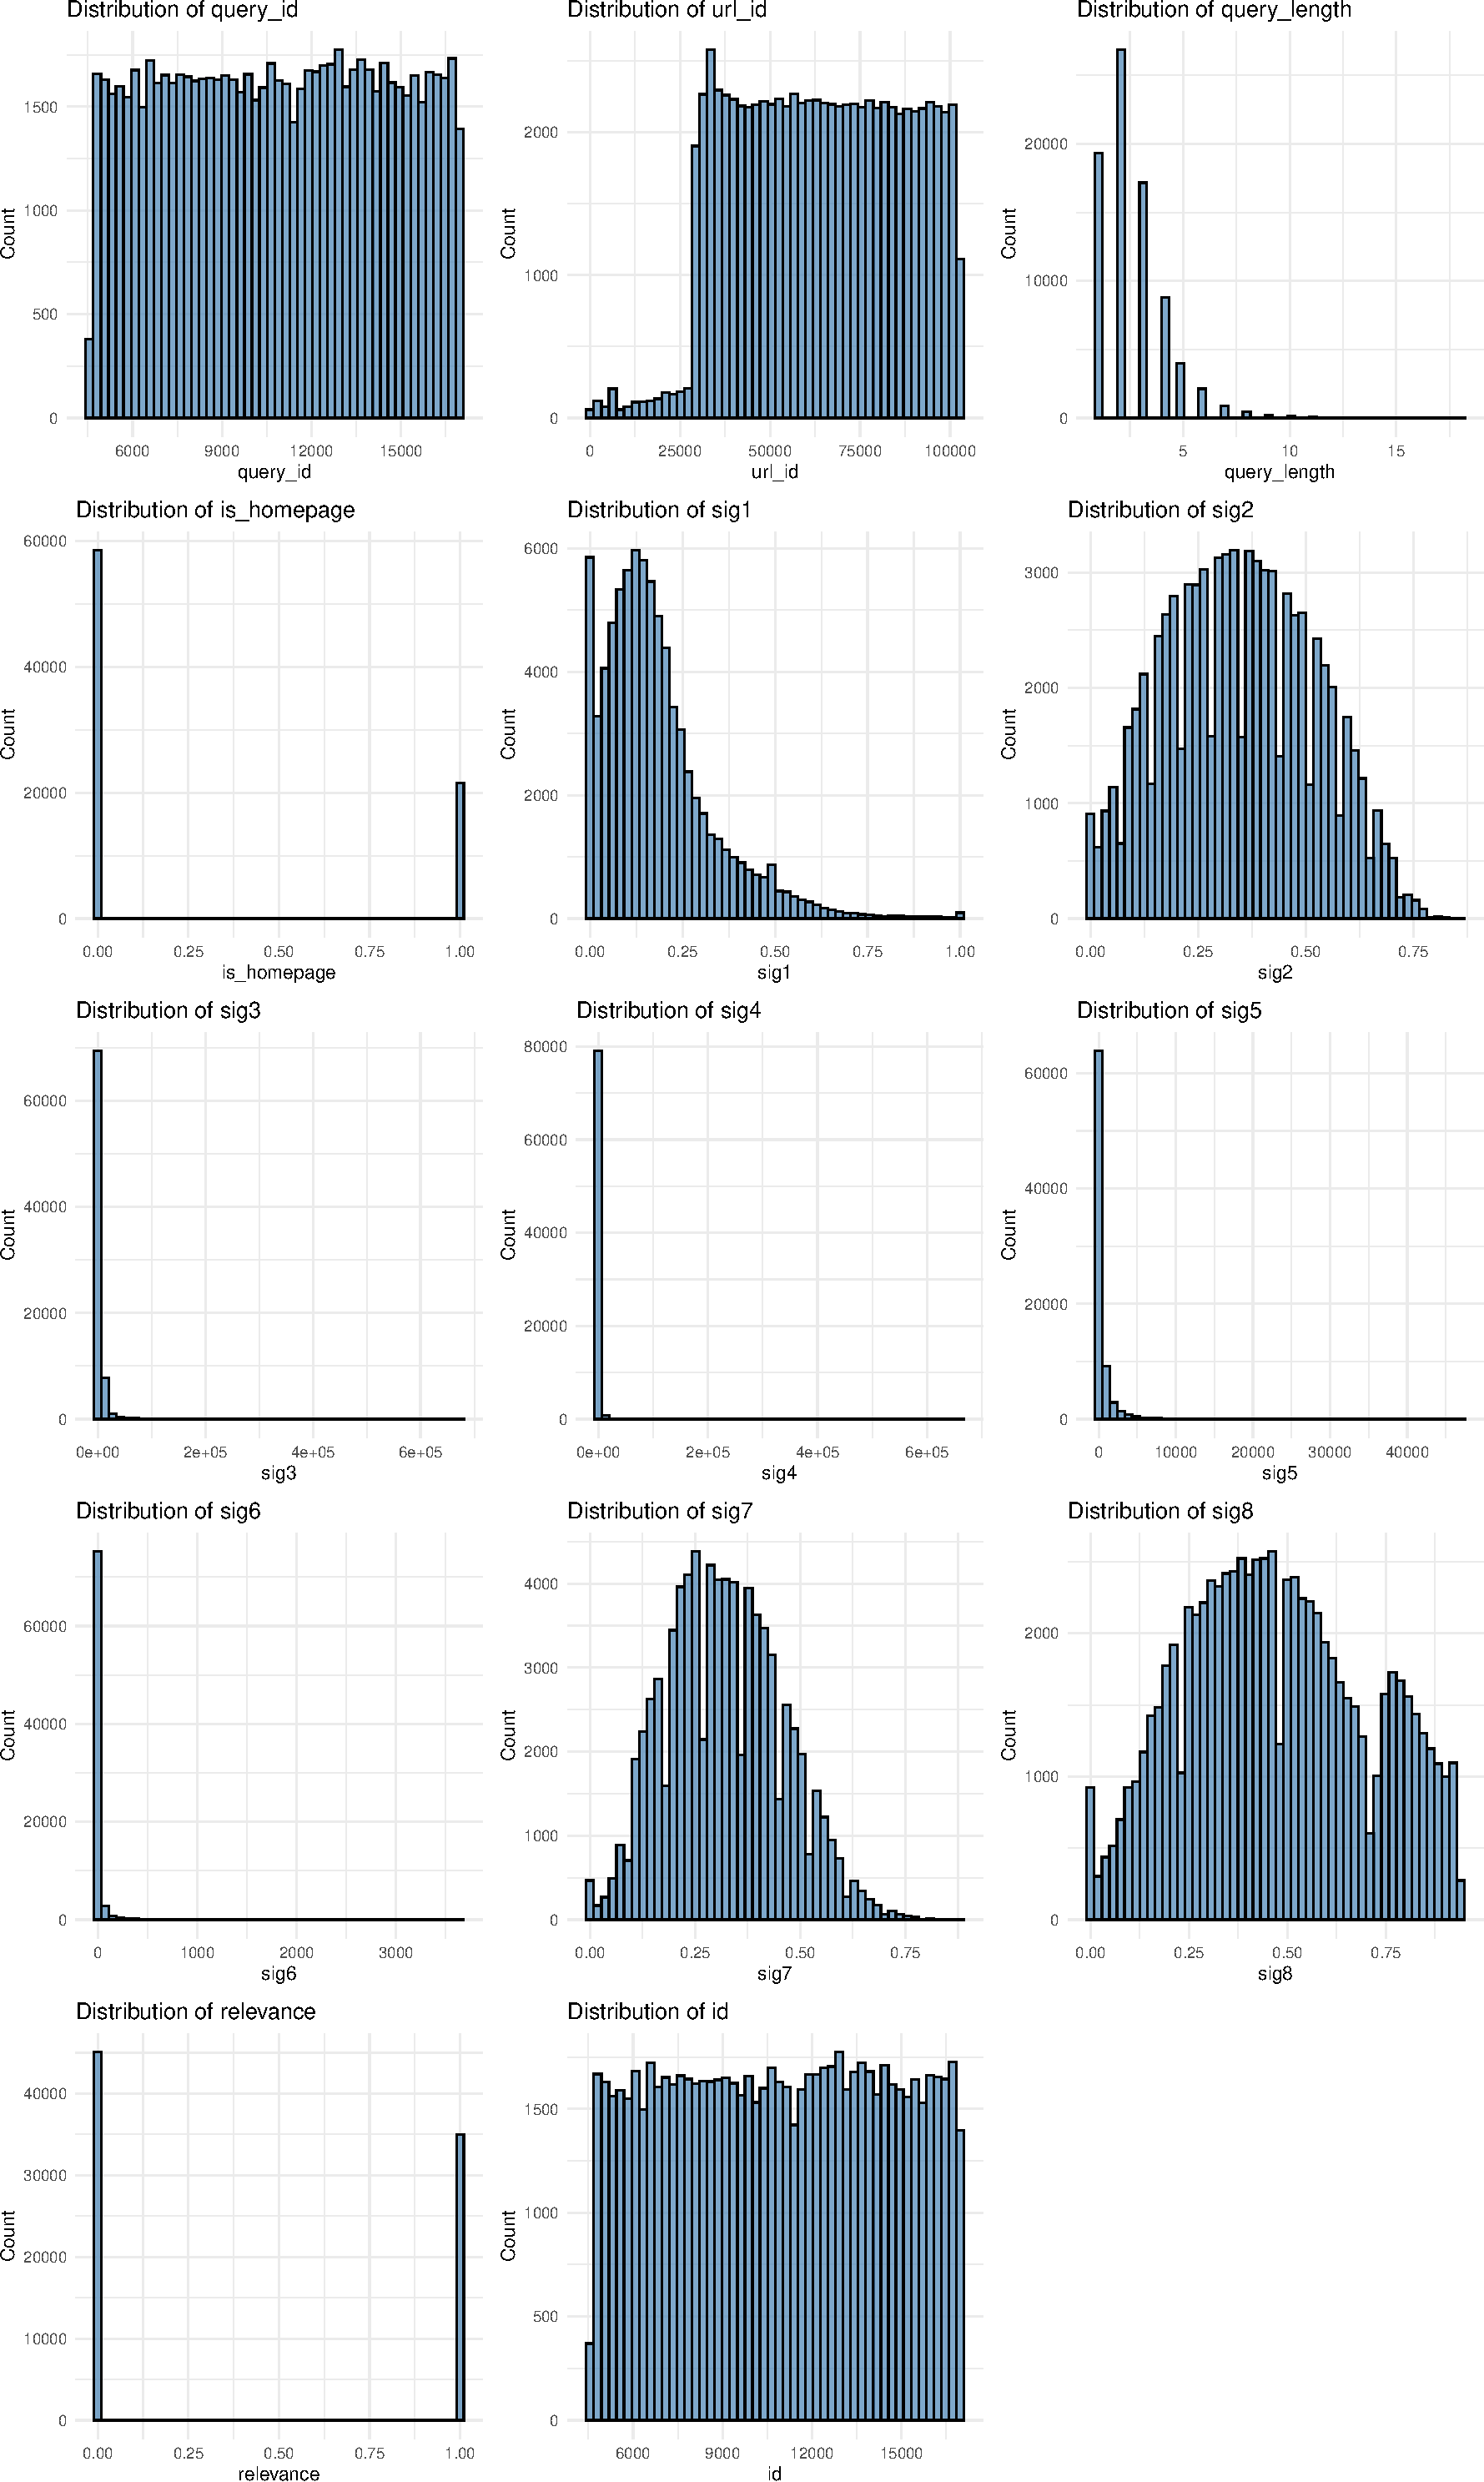
\includegraphics[keepaspectratio]{bue-alex-final-project_files/figure-pdf/unnamed-chunk-1-1.pdf}}

\paragraph{Histogram of Select Predictors Conditioned on Dependent
Variable}\label{histogram-of-select-predictors-conditioned-on-dependent-variable}

\pandocbounded{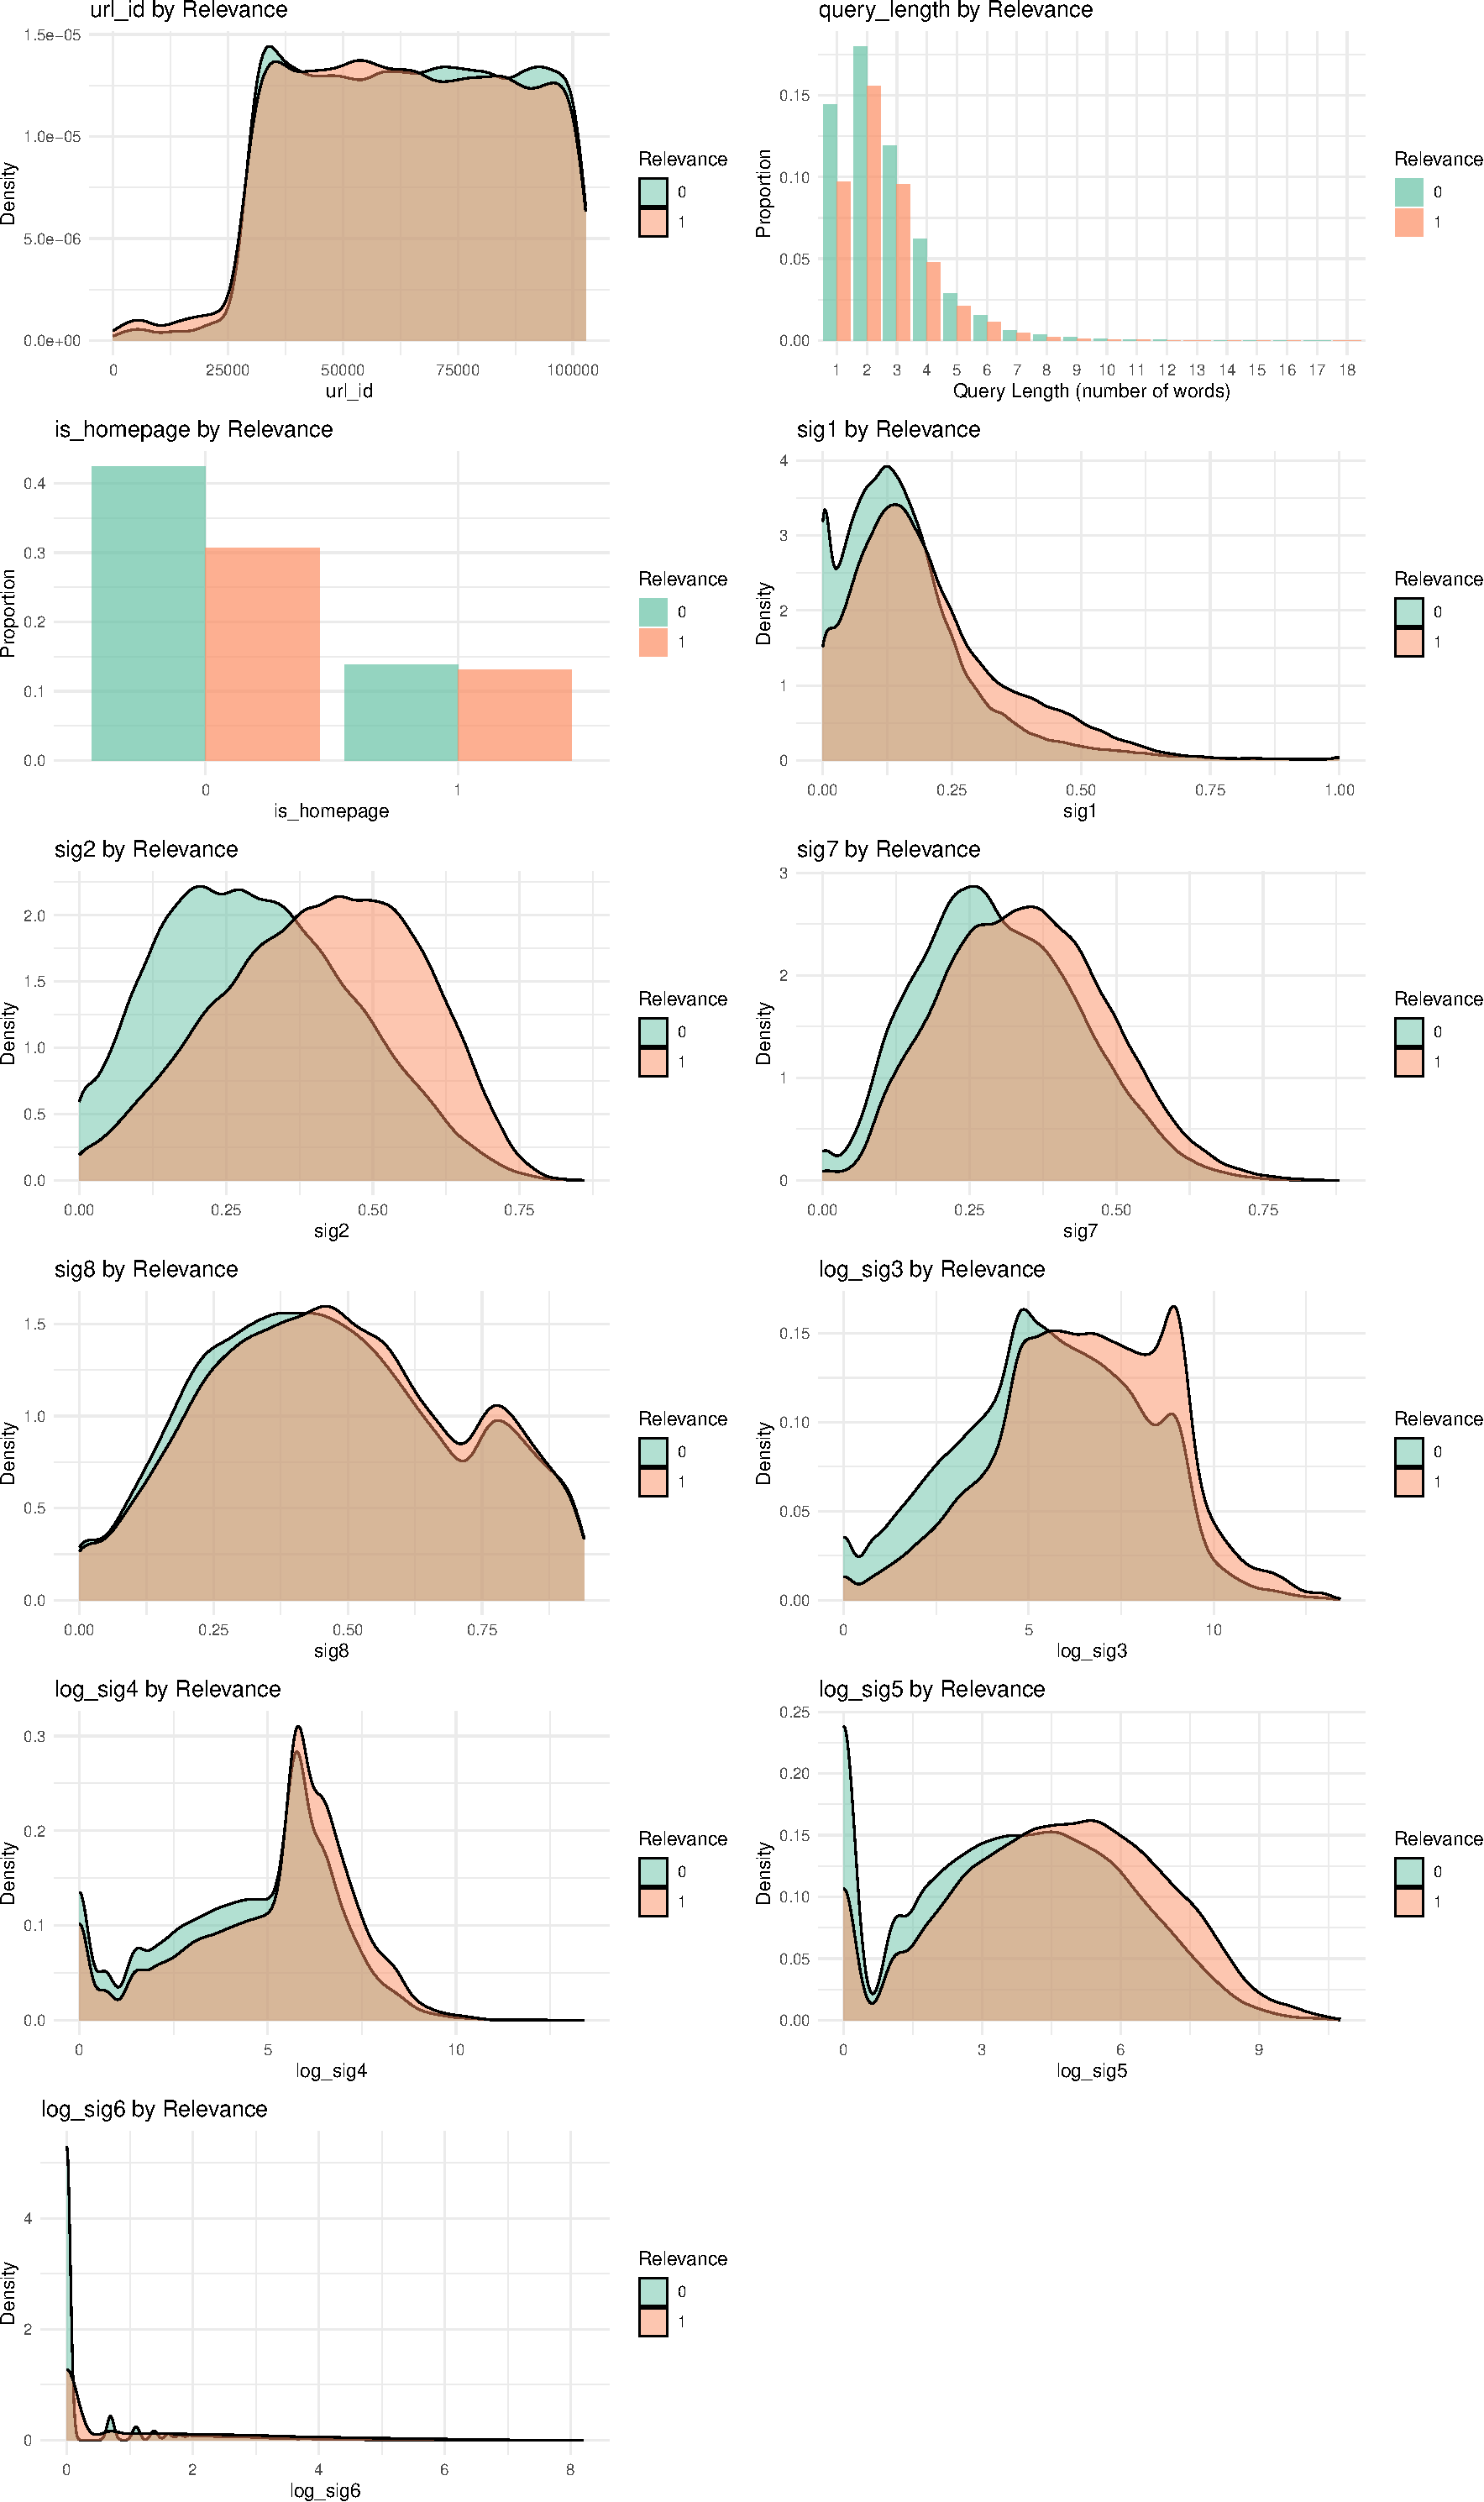
\includegraphics[keepaspectratio]{bue-alex-final-project_files/figure-pdf/unnamed-chunk-2-1.pdf}}

\paragraph{Proportions of Select Predictors Conditioned on Dependent
Variables
Deciles}\label{proportions-of-select-predictors-conditioned-on-dependent-variables-deciles}

\pandocbounded{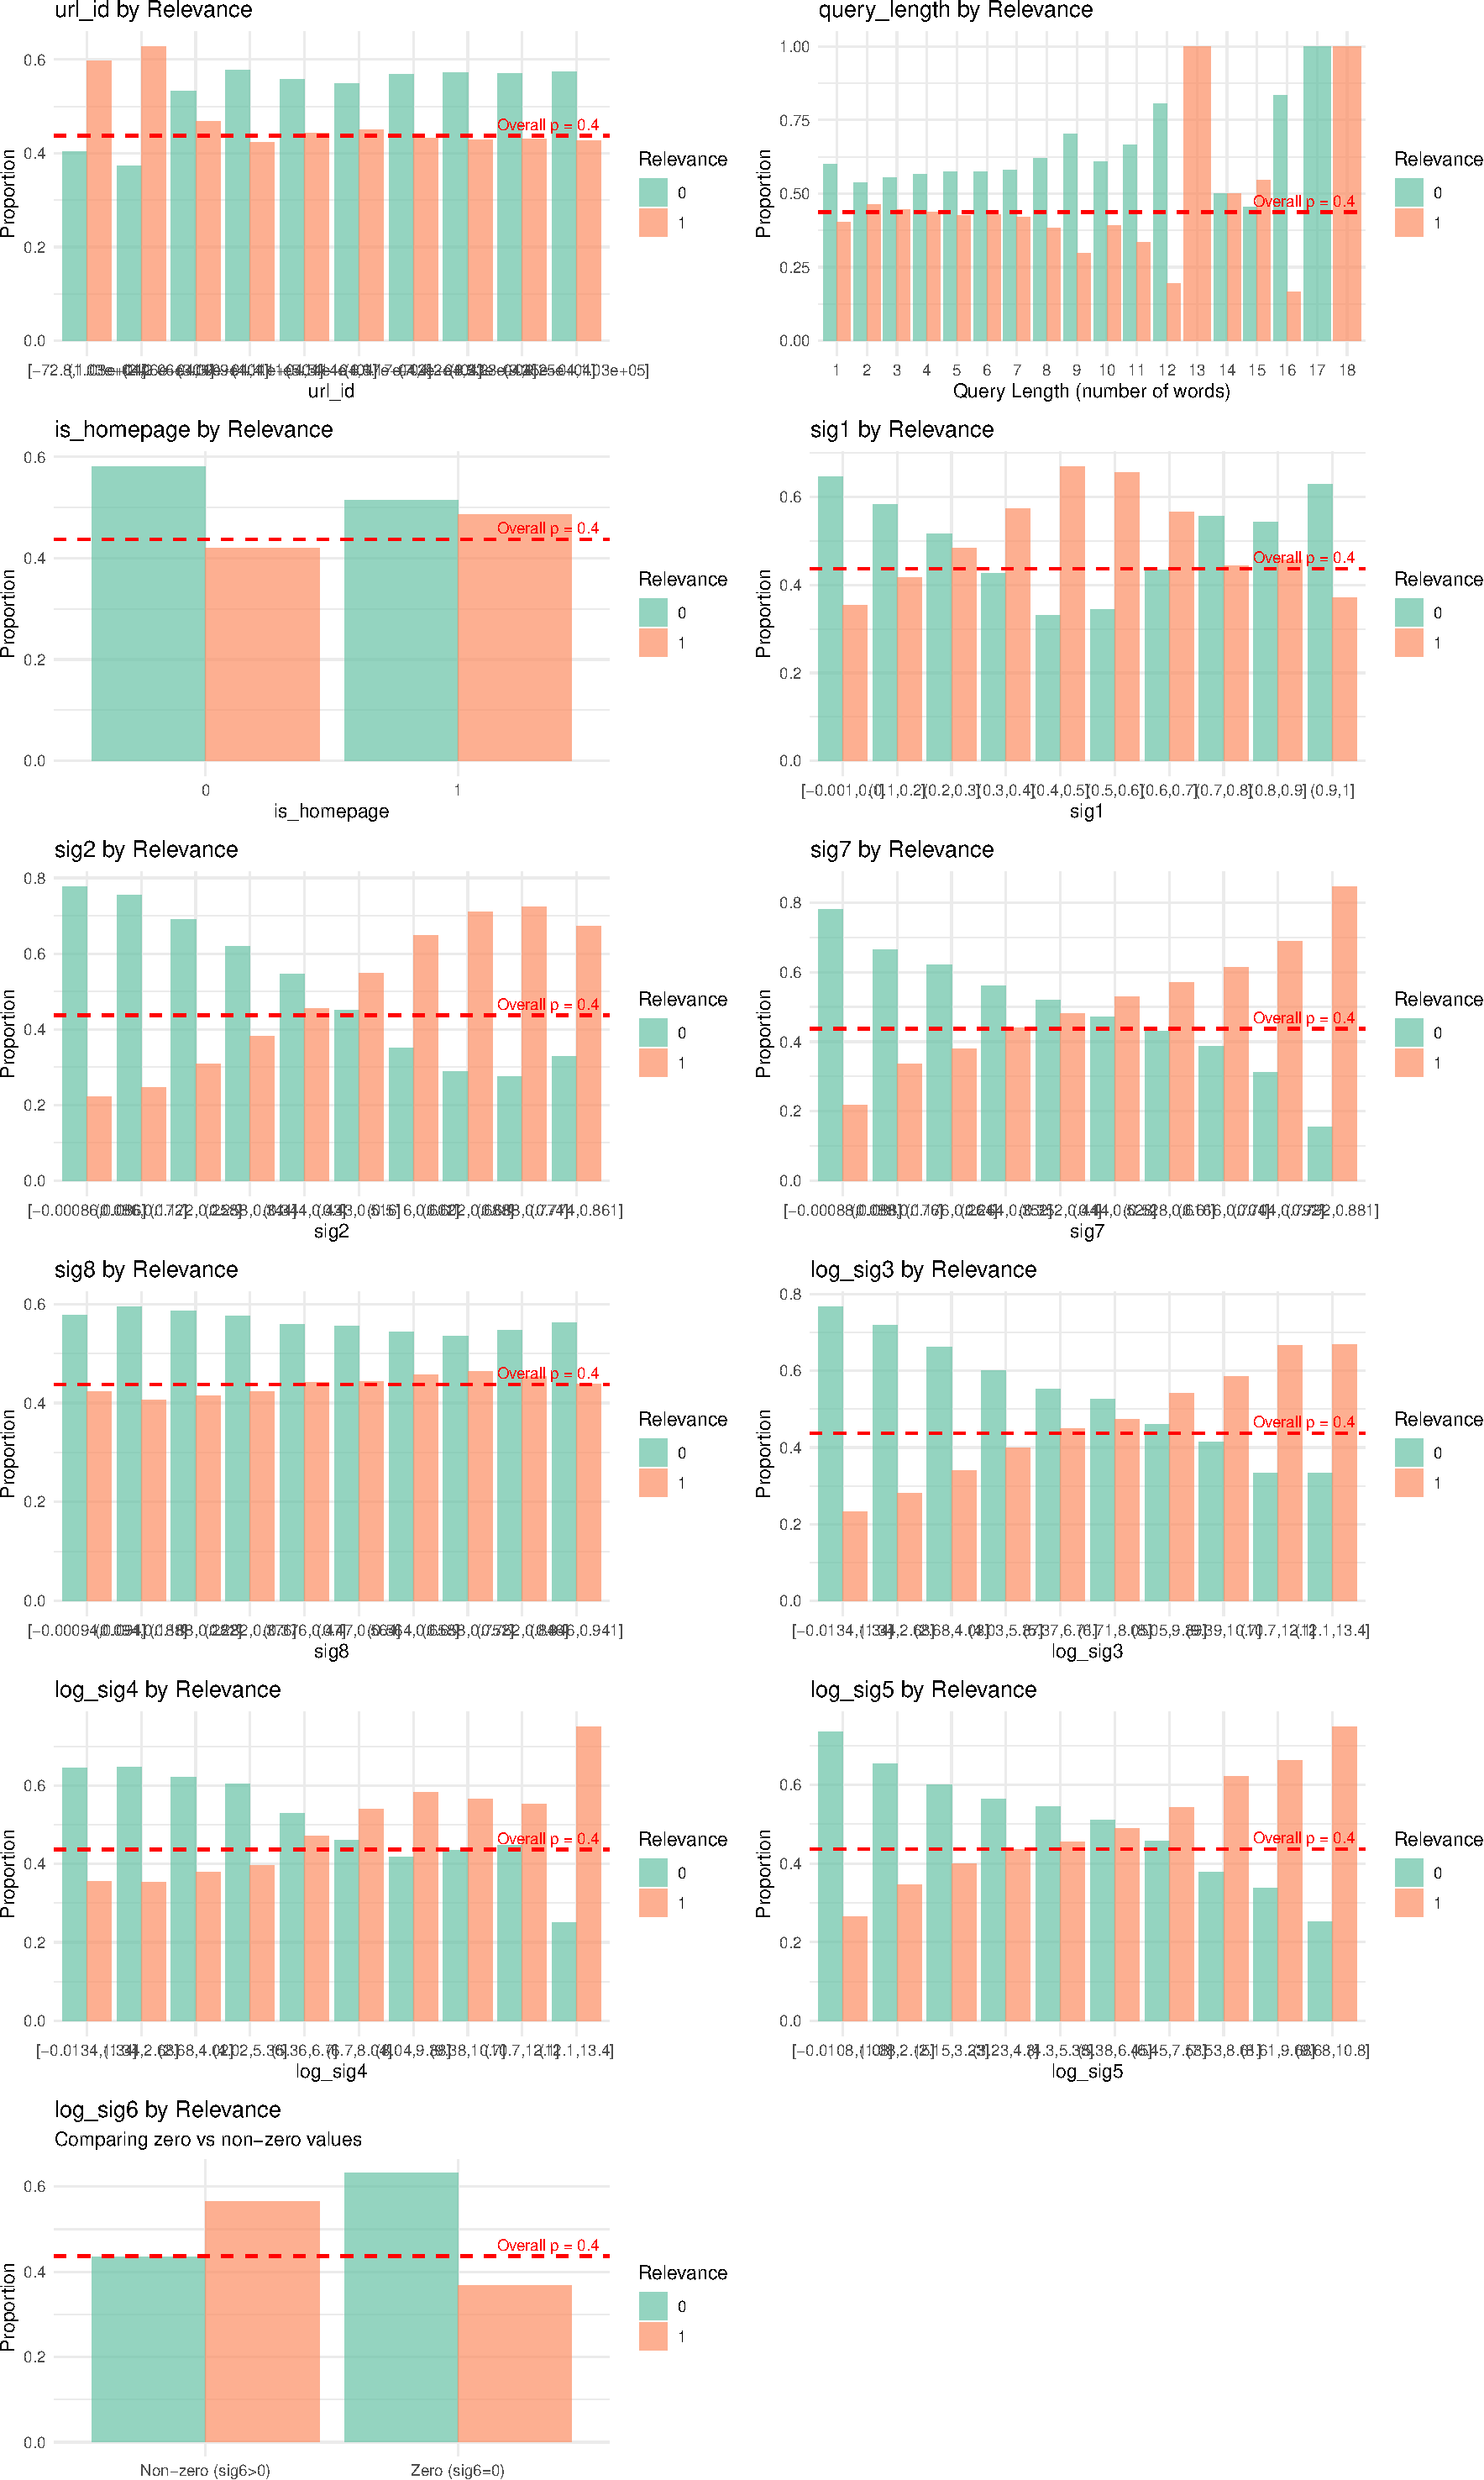
\includegraphics[keepaspectratio]{bue-alex-final-project_files/figure-pdf/unnamed-chunk-3-1.pdf}}

\paragraph{Correlation Plot}\label{correlation-plot}

\pandocbounded{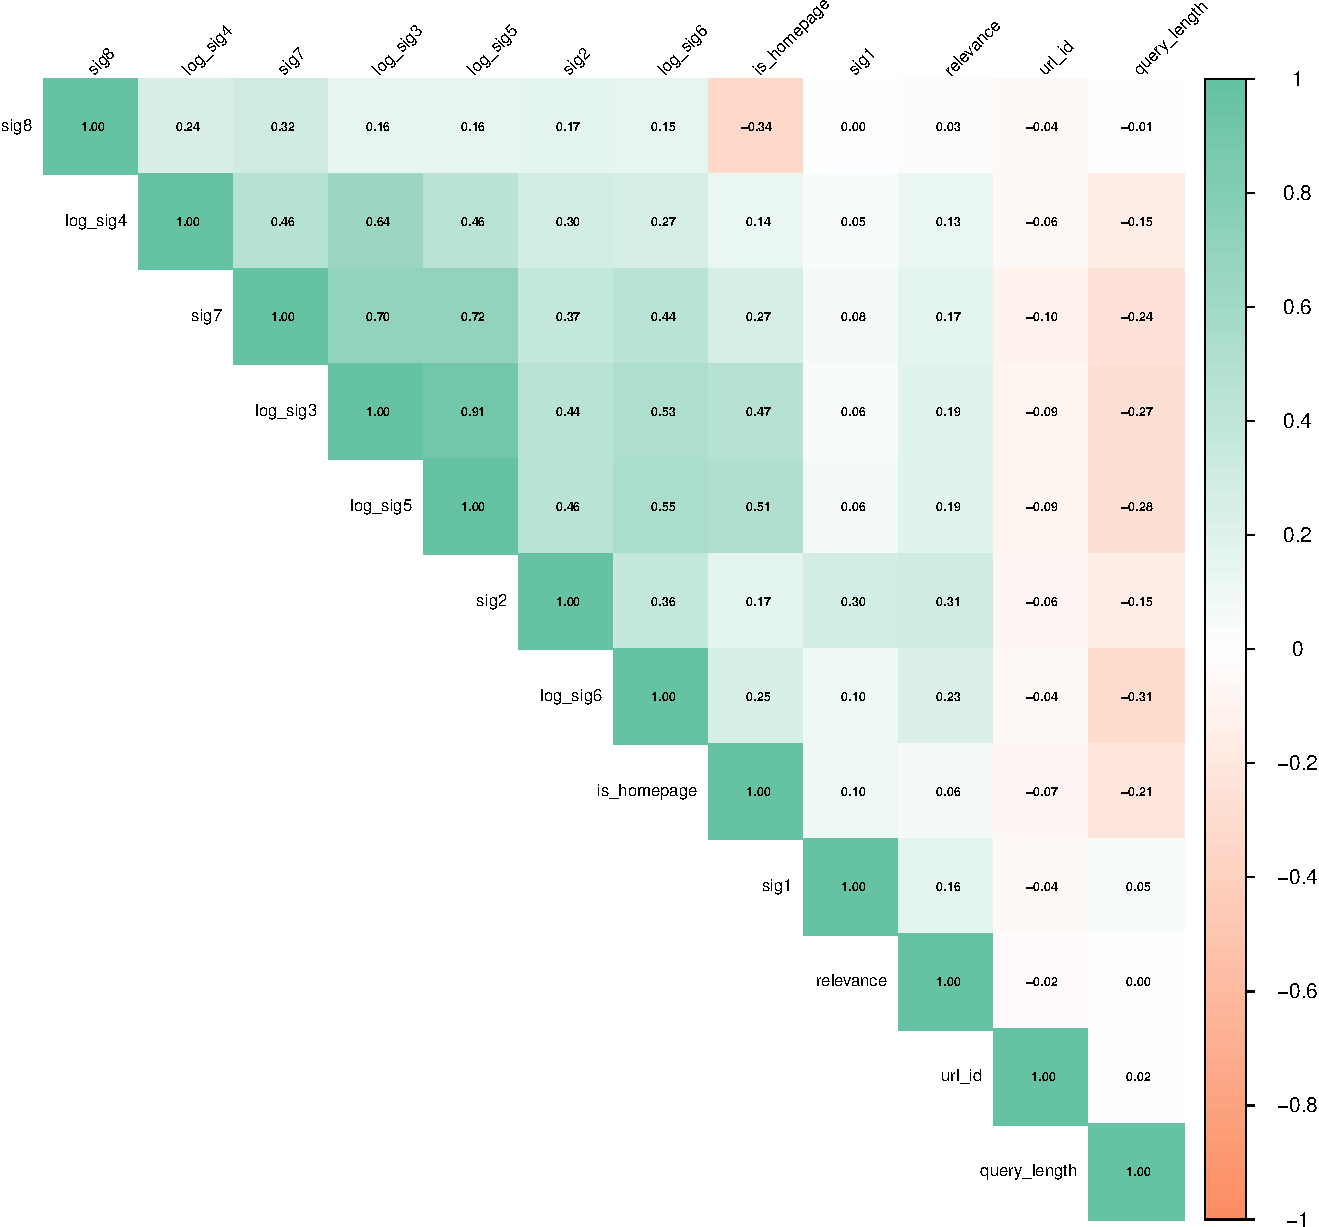
\includegraphics[keepaspectratio]{bue-alex-final-project_files/figure-pdf/unnamed-chunk-4-1.pdf}}

\paragraph{Query Length}\label{query-length}

Longer query lengths have a very high proportion of relevant entries. I
calculate standard errors to see whether these trends are statistically
significant or may result in over-fitting.

\pandocbounded{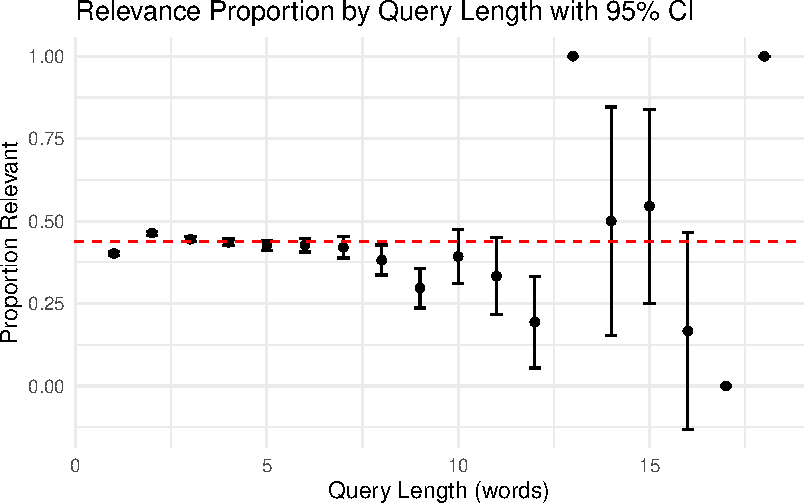
\includegraphics[keepaspectratio]{bue-alex-final-project_files/figure-pdf/unnamed-chunk-5-1.pdf}}

They are not statistically significant.

\subsubsection{URL ID}\label{url-id}

\pandocbounded{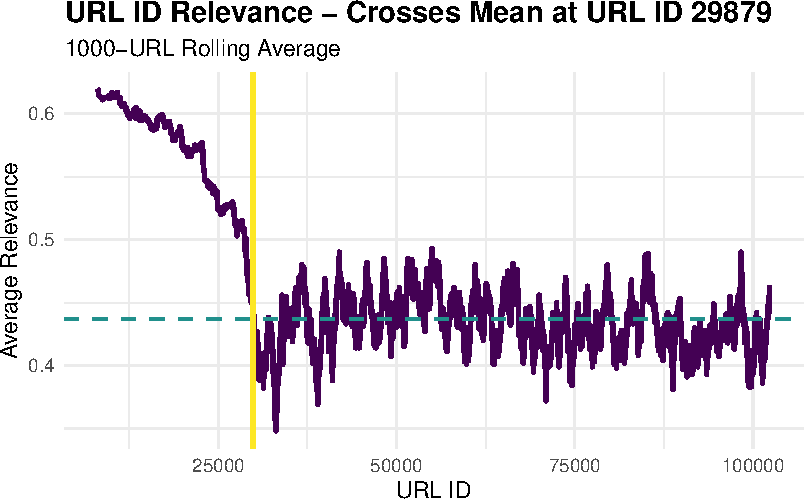
\includegraphics[keepaspectratio]{bue-alex-final-project_files/figure-pdf/unnamed-chunk-6-1.pdf}}

\subsection{Pre-processing}\label{pre-processing}

I code \texttt{is\_homepage} as an unordered factor.

I remove \texttt{query\_length} because the most predictive lengths are
also the most rare. It is sensible to represent \texttt{query\_length}
as a factor variable, because the proportion of relevance does not
appear to increase linearly, but factors introduce various challenges
with prediction. If some factor is not present in the future data, then
our trained model will not work. A compromise is necessary.

\texttt{url\_id} will need to be handled differently. The numeric scale
is not sensible but neither are factors, which would lead to
over-fitting. Ultimately, it seems risky to include data that may be
idiosyncratic, but I retain it because the stakes here are relatively
low.

\texttt{sig2,\ sig7,\ and\ sig8} appear to have regular drop-offs in the
histograms. This is an artifact of the measurement scale, which records
values in increments of \(0.01\). Some histogram bins therefore align
with the allowed values and receive higher counts, while others fall
between these values and receive few or none, producing the visible
pattern of regular dips. This is not a problem for analysis.

There are no missing values.

\subsection{Transformation}\label{transformation}

I apply the following transformations:

\begin{itemize}
\tightlist
\item
  Log-transform skewed variables (\texttt{sig3,\ sig4,\ sig5}) for
  linear models.

  \begin{itemize}
  \tightlist
  \item
    This linearizes for LASSO, and monotone transformations are unlikely
    to hurt more flexible modeling strategies.
  \item
    I use \texttt{log1p} from base R, which adds a constant of \(1\) to
    each value to avoid issues with zeros. The loss of the usual
    interpretability - where natural logs approximate percentage changes
    - is not important here.
  \end{itemize}
\item
  Two-part transformation for \texttt{sig6}: create a dummy variable
  indicating zero values, then log-transform the positive values. This
  preserves the information in zeros (which show a higher proportion of
  relevance) while making the positive values less skewed.
\item
  I add binary variables for \texttt{query\_length} 1 and 2, which are
  statistically significant according to my earlier visualization.
\item
  I add a factor variable for \texttt{url\_id} below \(30000\), the
  cutoff at which mean relevance was highest.
\item
  After transforming, I remove \texttt{url\_id} and other variables.
\end{itemize}

Note that I do not standardize at this stage. Since I will later use
cross-validation, scaling of the variables should happen within each
fold where appropriate.

\begin{longtabu} to \linewidth {>{\raggedright}X>{\centering}X>{\raggedright}X>{\raggedright}X}
\caption{\label{tab:unnamed-chunk-9}Summary of Transformed Variables for Modeling}\\
\toprule
Variable & Type & Description & Transformation\\
\midrule
relevance & Binary & Target variable (0 = not relevant, 1 = relevant) & None\\
is\_homepage & Factor & Whether the URL is a homepage & Factor\\
sig1 & Continuous & Original signal feature 1 & None\\
sig2 & Continuous & Original signal feature 2 & None\\
log\_sig3 & Continuous & Log-transformed sig3 & log1p(sig3)\\
\addlinespace
log\_sig4 & Continuous & Log-transformed sig4 & log1p(sig4)\\
log\_sig5 & Continuous & Log-transformed sig5 & log1p(sig5)\\
sig6\_is\_zero & Binary & Indicator for sig6 = 0 & sig6 == 0\\
log\_sig6\_positive & Continuous & Log of sig6 when positive & log(sig6) if sig6 > 0\\
sig7 & Continuous & Original signal feature 7 & None\\
\addlinespace
sig8 & Continuous & Original signal feature 8 & None\\
single\_word\_query & Binary & Query length = 1 & query\_length == 1\\
two\_word\_query & Binary & Query length = 2 & query\_length == 2\\
three\_word\_query & Binary & Query length = 3 & query\_length == 3\\
low\_url\_id & Binary & URL ID < 30000 & url\_id < 30000\\
\bottomrule
\end{longtabu}

\subsection{Data Mining}\label{data-mining}

I will use 10-fold cross-validation to estimate generalization error for
each modeling strategy. In all cases, I will evaluate model accuracy,
picking the tuning parameters and then the strategy which maximizes
accuracy.

My modeling strategies are:

\begin{enumerate}
\def\labelenumi{\arabic{enumi}.}
\tightlist
\item
  LASSO logistic regression: Suitable for correlated predictors and
  sparse data to reduce variance. Factor variables are one-hot encoded.
  The tuning variable is \(\lambda\), imposing a progressively higher
  penalty that shrinks coefficients towards zero. I use a
  ``kitchen-sink'' approach with all interactions.
\item
  KNN: A simple, intuitive method that makes minimal assumptions about
  the data's functional form. Factor variables are one-hot encoded; the
  curse of dimensionality is not salient given the relatively low
  dimensions. The tuning variable is \(k\), or the number of nearest
  neighbors.
\item
  Random Forests: Well-suited to low-dimensional tabular data and
  capable of capturing complex, nonlinear interactions automatically
  without needing the earlier transformations; especially attractive
  given apparent splines in some variables (\texttt{sig1}). Factor
  variables are not one-hot encoded because one-hot encoding increases
  the number of predictors, resulting in over-representation of factor
  variables by random forests. The tuning parameters are below:
\end{enumerate}

\begin{Shaded}
\begin{Highlighting}[]
\NormalTok{rf\_grid }\OtherTok{\textless{}{-}} \FunctionTok{expand.grid}\NormalTok{(}
  \AttributeTok{mtry =} \FunctionTok{c}\NormalTok{(}\DecValTok{2}\NormalTok{, }\DecValTok{4}\NormalTok{, }\DecValTok{6}\NormalTok{, default\_mtry),}
  \AttributeTok{splitrule =} \StringTok{"gini"}\NormalTok{,}
  \AttributeTok{min.node.size =} \FunctionTok{c}\NormalTok{(}\DecValTok{1}\NormalTok{, }\DecValTok{5}\NormalTok{, }\DecValTok{10}\NormalTok{)}
\NormalTok{)}
\end{Highlighting}
\end{Shaded}

\begin{enumerate}
\def\labelenumi{\arabic{enumi}.}
\setcounter{enumi}{3}
\tightlist
\item
  I also use gradient boosting with XGBoost. The tuning parameters are
  below:
\end{enumerate}

\begin{Shaded}
\begin{Highlighting}[]
\NormalTok{cv }\OtherTok{\textless{}{-}} \FunctionTok{xgb.cv}\NormalTok{(}
  \AttributeTok{params =}\NormalTok{ params,}
  \AttributeTok{data =}\NormalTok{ dtrain,}
  \AttributeTok{nrounds =} \DecValTok{150}\NormalTok{,}
  \AttributeTok{nfold =} \DecValTok{10}\NormalTok{,}
  \AttributeTok{early\_stopping\_rounds =} \DecValTok{10}\NormalTok{,}
  \AttributeTok{verbose =} \ConstantTok{FALSE}
\NormalTok{)}
\end{Highlighting}
\end{Shaded}

Computational constraints limit somewhat my range of tuning parameters.
I do not tune probability thresholds, though this would be an obvious
next step in my analysis. Boosting could be tuned with more options, not
just the number of rounds.

\subsection{Interpretation/Evaluation}\label{interpretationevaluation}

Boosting with XGBoost performs the best.

LASSO keeps many variables. The coefficients represent changes in the
log odds ratio but analysts are discouraged from making inferences about
them; it is a known feature of penalized regressions that correlated
covariates may be included in the final model without having an
underlying causal effect on the dependent variable.

The random forests model uses a generic 500 trees. \texttt{sig2} is the
most important feature. When \texttt{sig2} is permuted, the model's
accuracy drops the most compared to any other predictor, so the forest
relies heavily on it for splitting and prediction.

These results generally concur with the earlier visualizations.
\texttt{sig2} appeared to uniquely partition dependent and independent
variables.

Below is a table summarizing results, followed by visualizations of each
modeling strategy's variable selection methods and performance.

\begin{longtable}[t]{lcl}
\caption{\label{tab:unnamed-chunk-10}Model Performance Comparison}\\
\toprule
Model & CV Accuracy & Optimal Parameters\\
\midrule
LASSO & 0.66605 & λ = 1e-04\\
KNN & 0.66600 & k = 149\\
Random Forest & 0.66614 & mtry = 3\\
\cellcolor[HTML]{4CAF50}{\textcolor{white}{\textbf{XGBoost}}} & \cellcolor[HTML]{4CAF50}{\textcolor{white}{\textbf{0.66737}}} & \cellcolor[HTML]{4CAF50}{\textcolor{white}{\textbf{iterations = 46}}}\\
\bottomrule
\end{longtable}

\subsubsection{LASSO}\label{lasso}

\begin{longtable}[t]{l>{}r}
\caption{\label{tab:unnamed-chunk-11}Head of LASSO Selected Features (91 variables + intercept)}\\
\toprule
Feature & Coefficient\\
\midrule
\textbf{sig2} & \textcolor{darkgreen}{\textbf{2.8803}}\\
is\_homepage1:sig7 & \textcolor{darkred}{-1.7308}\\
(Intercept) & \textcolor{darkred}{-1.5162}\\
sig1:sig7 & \textcolor{darkred}{-1.4295}\\
sig7:sig8 & \textcolor{darkred}{-1.3312}\\
\addlinespace
is\_homepage1:sig1 & \textcolor{darkgreen}{1.3215}\\
\bottomrule
\end{longtable}

\pandocbounded{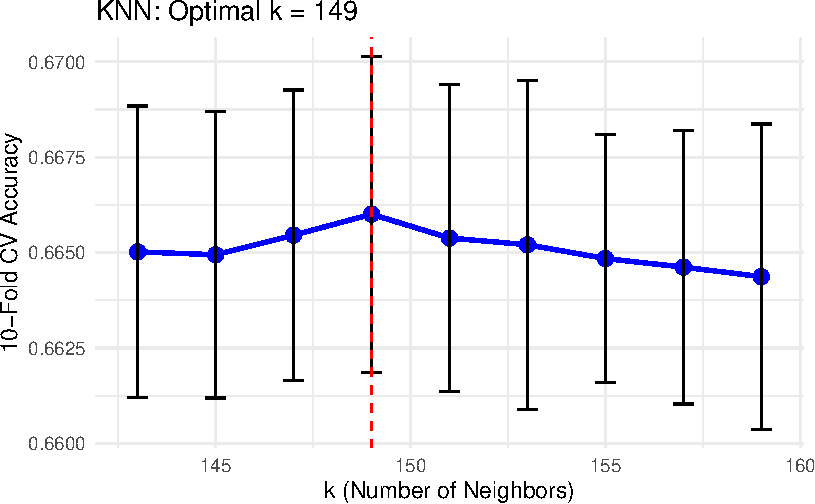
\includegraphics[keepaspectratio]{bue-alex-final-project_files/figure-pdf/unnamed-chunk-11-1.pdf}}

\subsubsection{KNN}\label{knn}

\pandocbounded{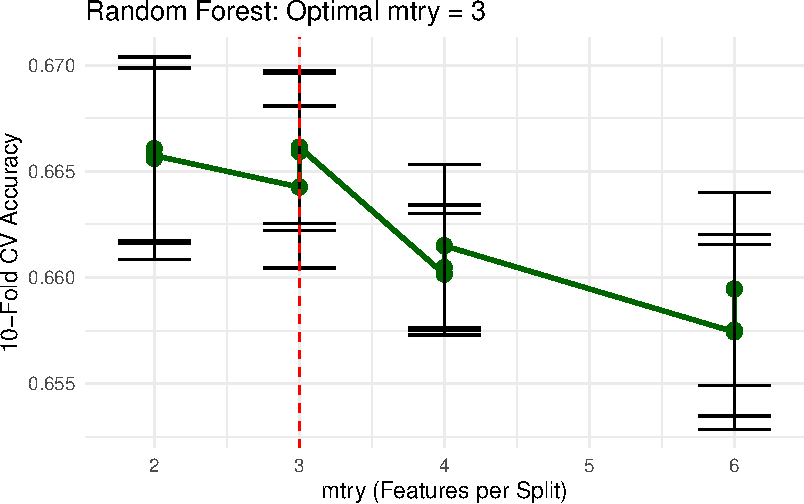
\includegraphics[keepaspectratio]{bue-alex-final-project_files/figure-pdf/unnamed-chunk-12-1.pdf}}

\subsubsection{Random Forests}\label{random-forests}

\pandocbounded{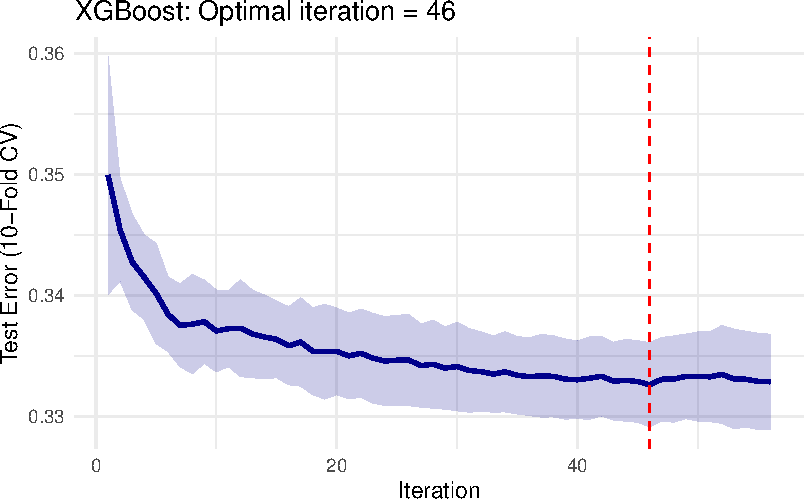
\includegraphics[keepaspectratio]{bue-alex-final-project_files/figure-pdf/unnamed-chunk-13-1.pdf}}

\pandocbounded{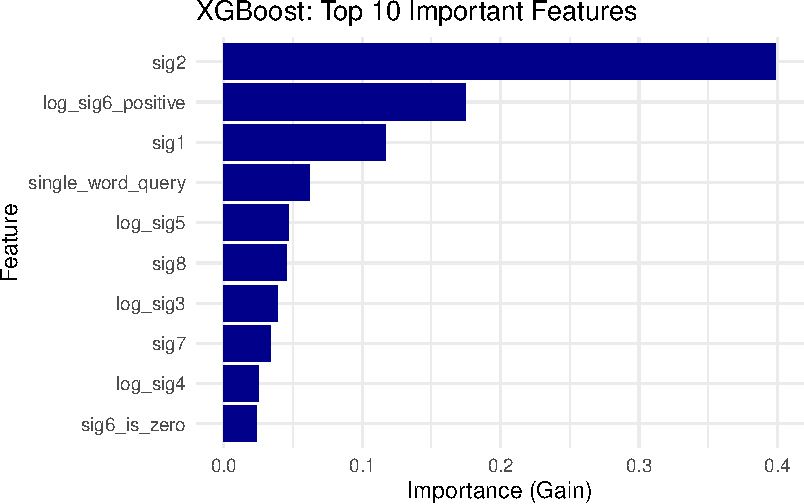
\includegraphics[keepaspectratio]{bue-alex-final-project_files/figure-pdf/unnamed-chunk-13-2.pdf}}

\subsubsection{XGBoost}\label{xgboost}

\pandocbounded{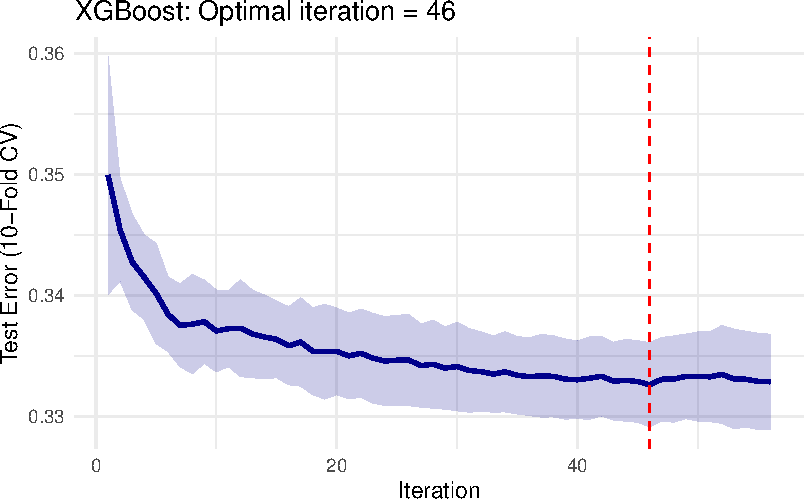
\includegraphics[keepaspectratio]{bue-alex-final-project_files/figure-pdf/unnamed-chunk-14-1.pdf}}

\pandocbounded{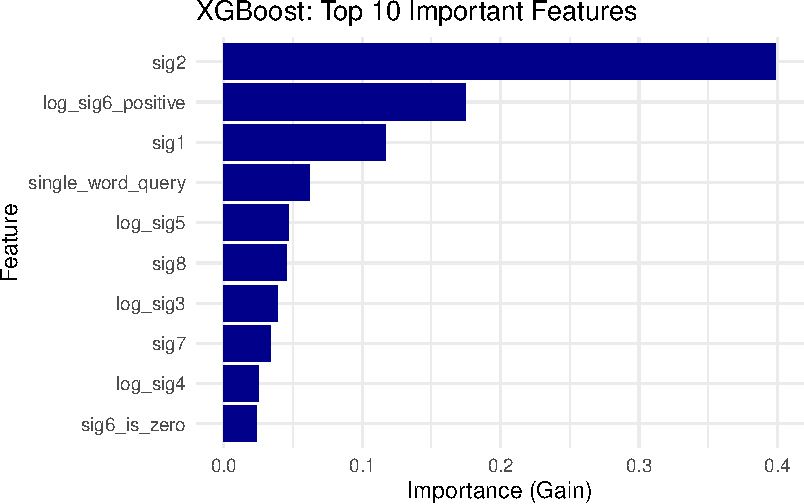
\includegraphics[keepaspectratio]{bue-alex-final-project_files/figure-pdf/unnamed-chunk-14-2.pdf}}

\subsection{Testing}\label{testing}

A script for creating the test submissions is included in the GitHub
Repository: https://github.com/24-bee-supply/stats-202-project.

\subsection{Conclusion}\label{conclusion}

This was an instructive project. Textbooks, forums, and large language
models have lowered the barriers to using the sophisticated data-mining
techniques from this class. Most students' results were relatively
similar, but the top performers tended to share two strategies:

\begin{enumerate}
\def\labelenumi{\arabic{enumi}.}
\tightlist
\item
  They engineered new features.
\item
  They iterated on their initial best-performing model.
\end{enumerate}

My approach was more modest. I prioritized visualizing the data to
better understand its functional form. I had assumed this emphasis would
be relatively unique given the temptation to simply train a large,
powerful neural network. But my efforts were incomplete. The
log-transformations I applied, as noted earlier, theoretically mattered
for linear models but not for more flexible ones. My attempts to find
``signal'' in the noise through data exploration should have been more
analytical and model-agnostic. Including \texttt{url\_id} was also
almost certainly a mistake.

This experience highlights areas where I am eager to grow as a data
scientist, particularly in embeddings, careful attention to the test
data distribution, and quantifying over-fitting.

Dr.~Tranh helped solidify a critical but, until recently,
under-appreciated concept for me: it is important to make learning as
easy as possible for the model. Powerful, flexible modeling strategies
do not remove the need to understand and thoughtfully shape your data so
that the problem is better-conditioned. Statistically, sprawling and
complex models may achieve low bias but often at the cost of high
variance, a pattern evident in the Kaggle competition's private scores.
Every machine learning course covers the bias-variance decomposition,
but recognizing why simplicity matters in practice is, I think, a
hallmark of mature modeling. Of course, it is also possible that I am
wrong and complexity often pays. This is an area I am excited to
explore.

Dr.~Tranh's emphasis on understanding your test data, even gaming the
system if possible, was another important lesson. At various points in
my analysis, especially involving the \texttt{url\_id} and
\texttt{query\_length} variables, it occurred to me that certain
assumptions might not generalize. Dogmatically, I refused to model the
test data, but in real-world applications it is important to investigate
whether your training data actually resembles the test data.

Finally, I am eager to learn more about learning curves and other
diagnostics of over-fitting. It is easy to run cross-validation,
optimize a loss function, and conclude that a model is adequate. I want
to go further---developing analyses that quantify over-fitting and
pinpoint how and where a model fails compared to alternatives. For
example, the team that won the first stage of the competition but lost
the second likely relied on cross-validation to estimate generalization
error, yet their model underperformed against one that remained
consistent across both stages. I want to understand and apply
diagnostics that can detect such issues, even when the modeling process
appears rigorous.




\end{document}
